\section[Unsupervised ML]{Unsupervised machine learning for text}


\question{Recap: Can you explain the difference between supervised and unsupervised machine learning?}


\begin{frame}{Remember the two flavours:}

\begin{enumerate}
\item Finding similar variables (dimension reduction)
\item Finding similar cases (clustering)
\end{enumerate}

\pause

Are we more interested in which features ``belong together'' or which cases ``belong together''? 

\end{frame}


\begin{frame}{We could use PCA/SCD\ldots}
  \ldots and try to understand which ``variables'' (== columns == words) cooccur

  Remember:
\begin{itemize}
\item Components are ordered (first explains most variance)
\item Components do \emph{not} necessarily carry a meaningful interpretation
\end{itemize}
\end{frame}




\begin{frame}[fragile,plain]{}
  \begin{minted}{python}
from sklearn import datasets
from sklearn.decomposition import TruncatedSVD
from sklearn.feature_extraction.text import TfidfVectorizer
from sklearn.pipeline import make_pipeline

texts = datasets.fetch_20newsgroups(data_home='rec.autos', remove=('headers', 'footers', 'quotes'), subset='train')['data']

myvec = TfidfVectorizer(max_df=.5, min_df=5, token_pattern='(?u)\\b[a-zA-Z][a-zA-Z]+\\b')
mysvd = TruncatedSVD(n_components=3)
mypipe = make_pipeline(myvec, mysvd)
r = mypipe.fit_transform(texts)
\end{minted}
\end{frame}





\begin{frame}[fragile]{Plotting the texts according to their component scores}
\begin{lstlisting}
import matplotlib.pyplot as plt

fig = plt.figure(figsize=(10,10))
ax = fig.add_subplot(projection='3d')
ax.scatter([e[0] for e in r], [e[1] for e in r],  [e[2] for e in r],alpha=.2)
\end{lstlisting}

\makebox[\linewidth]{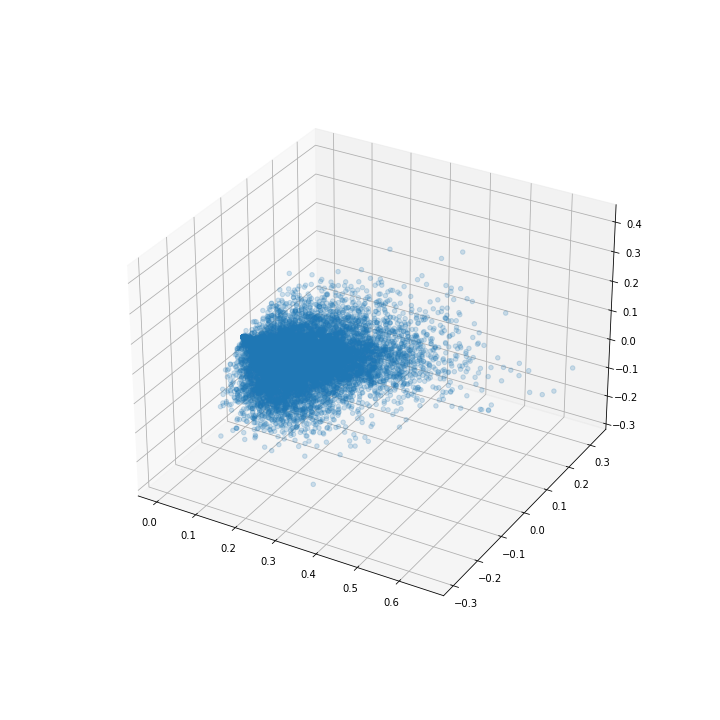
\includegraphics[width=\paperwidth,height=.6\paperheight,keepaspectratio]{svd3d}}

\end{frame}



\begin{frame}[fragile]{Using the scores}
\begin{lstlisting}
import pandas as pd
textscores= pd.DataFrame(r)
featurescores = pd.DataFrame(mysvd.components_.T, index = myvec.get_feature_names())
\end{lstlisting}

\makebox[\linewidth]{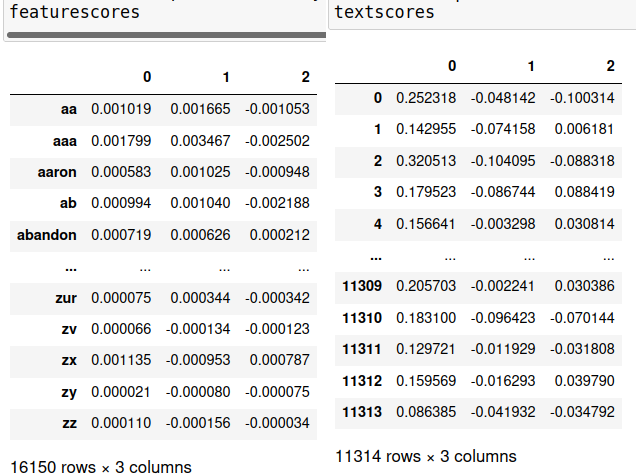
\includegraphics[width=\paperwidth,height=.6\paperheight,keepaspectratio]{svdscores}}

\end{frame}



\begin{frame}{Grouping features vs grouping cases}
  We have a  corpus of a many texts.
  
\begin{itemize}
\item We used SVD to figure out relationships between features
\item We could now look at the most important features per component (``topic'', ``frame''?) by sorting \texttt{featurescores}
\item We could see which texts are most representative for each ``topic'' or ``frame'' by sorting \texttt{textscores}
\end{itemize}
\pause

$\Rightarrow$ Alternative: Choose the opposite approach and first find out which cases are most similar, \textit{then} describe what features characterize each group of cases


\end{frame}





\begin{frame}[plain,fragile]
\begin{minted}{python}
from sklearn.cluster import KMeans

k = 5

mykm = KMeans(n_clusters=k, init='k-means++', max_iter=100, n_init=1)
myvec = TfidfVectorizer(max_df=.5, min_df=5, token_pattern='(?u)\\b[a-zA-Z][a-zA-Z]+\\b')
mypipe = make_pipeline(myvec, mykm)

predictions = mypipe.fit_transform(texts)
# potentially: textscores = pd.Dataframe(predictions)
\end{minted}

Of course, you need to determine the appropriate $k$\ldots (see earlier lecture)



\end{frame}


\begin{frame}[fragile,plain]{Let's get the terms closest to the centroids}
\begin{lstlisting}
order_centroids = mykm.cluster_centers_.argsort()[:, ::-1]
terms = myvec.get_feature_names()

print("Top terms per cluster:")

for i in range(k):
    print("Cluster {}: ".format(i), end='')
    for ind in order_centroids[i, :10]:
        print("{} ".format(terms[ind]), end='')
    print()

\end{lstlisting}
\pause
returns something like:

\begin{lstlisting}
Top terms per cluster:
Cluster 0: windows file dos window with on you this have files 
Cluster 1: you on this was with are have be not they 
Cluster 2: thanks any me have anyone or please if on this 
Cluster 3: he was his him not as this but on god 
Cluster 4: you are be not they as this have if on 
\end{lstlisting}
(of course, we could do sth similar with pandas as well)
\end{frame}






\begin{frame}{Let's summarize}
  \begin{itemize}
  \item Both PCA \parencite[e.g.][]{Greussing2017} and cluster analysis \parencite[e.g.,][]{burscher2016} have been used in the past to identify ``topics'' or ``frames''
  \item PCA groups features, cluster analysis groups texts
  \item (but you can then use the component scrores to describe the texts, and the cluster centroids to describe the features)
  \item Still ocasionally used, but in general considered outdated (for our use case)
  \end{itemize}

\end{frame}




\section[LDA]{From PCA and Clustering towards Latent Dirichlet Allocation (LDA)}


\begin{frame}{Let's assume we want to find out the topics in a large corpus of documents}
We could either
\begin{itemize}
	\item use PCA to find out related features (and interpret those as topics)
	\item or use clustering to find similar documents (and then look at the words they share to interpret as topics)
\end{itemize}

\pause

Actually, we have \emph{two} things we want to model:

\begin{enumerate}
	\item Which topics can we extract from the corpus?
	\item How present is each of these topics in each text in the corpus?
\end{enumerate}

\end{frame}


\begin{frame}[fragile]{Recap: PCA}
Document-term matrix
\begin{lstlisting}
      w1,w2,w3,w4,w5,w6 ...
text1, 2, 0, 0, 1, 2, 3 ...
text2, 0, 0, 1, 2, 3, 4 ...
text3, 9, 0, 1, 1, 0, 0 ...
...
\end{lstlisting}
{\small{These can be simple counts, but also more advanced metrics, like tf-idf scores (where you weigh the frequency by the number of documents in which it occurs), cosine distances, etc.}}
\pause
	\begin{itemize}
	\item given a term-document matrix, easy to do with any tool
	\item probably extremely skewed distributions
	\item some problematic assumptions: \textcolor{red}{does the goal of PCA, to find a solution in which one word loads on \emph{one} component match real life, where a word can belong to several topics or frames?}
\end{itemize}

\end{frame}


\begin{frame}{Recap: clustering}
\begin{itemize}
	\item given a term-document matrix, we can easily find clusters of documents that resemble each other
	\item but also here \textcolor{red}{does the goal of cluster analysis, assigning each document to \emph{one} cluster, match real life?}
\end{itemize}
\end{frame}


\begin{frame}{We need other models to}
\begin{enumerate}[<+->]
	\item model \emph{simultaneously} (a) which topics we find in the whole corpus, and (b) which of these topics are present in which document; while at the same time
	\item allowing (a) words to be part of multiple topics, and (b) multiple topics to be present in one document; and
	\item being able to make connections between words ``even if they never actually occured in a document together'' \parencite[p.~96]{Maier2018a}
\end{enumerate}

\end{frame}




\subsection{An introduction to LDA}

\begin{frame}{}
	Enter \textbf{topic modeling with Latent Dirichlet Allocation (LDA)}
\end{frame}






\begin{frame}{LDA, what's that?}
  \begin{block}{No mathematical details here, but the general idea}
    \begin{itemize}
    \item There are $k$ topics, $T_1$\ldots$T_k$
    \item Each document $D_i$ consists of a mixture of these topics, e.g.$80\% T_1, 15\% T_2, 0\% T_3, \ldots 5\% T_k $
    \item On the next level, each topic consists of a specific probability distribution of words
    \item Thus, based on the frequencies of words in $D_i$, one can infer its distribution of topics
    \item Note that LDA (like PCA) is a Bag-of-Words (BOW) approach
    \end{itemize}
  \end{block}
	
\end{frame}




\begin{frame}[fragile]{Doing a LDA in Python}
You can use gensim \cite{Rehurek2010} for this.

Let us assume you have a list of lists of words (!) called \texttt{texts}:

\begin{lstlisting}
articles=['The tax deficit is higher than expected. This said xxx ...', 'Germany won the World Cup. After a']
texts=[[token for token in re.split(r"\W", art) if len(token)>0] for art in articles]
\end{lstlisting}
which looks like this:
\begin{lstlisting}
[['The', 'tax', 'deficit', 'is', 'higher', 'than', 'expected', 'This', 'said', 'xxx'], ['Germany', 'won', 'the', 'World', 'Cup', 'After', 'a']]
\end{lstlisting}
(note that we of course could use a better tokenizer!)
\end{frame}




\begin{frame}[plain,fragile]
\begin{lstlisting}
from gensim import corpora, models
import pandas as pd

NTOPICS = 100
LDAOUTPUTFILE="topicscores.tsv"

# Create a BOW represenation of the texts
id2word = corpora.Dictionary(texts)
mm =[id2word.doc2bow(text) for text in texts]

# Train the LDA models.
mylda = models.ldamodel.LdaModel(corpus=mm, id2word=id2word, num_topics=NTOPICS, alpha="auto")

# Print the topics.
for top in mylda.print_topics(num_topics=NTOPICS, num_words=5):
  print ("\n",top)

# the topic scores per document
topics = pd.DataFrame([dict(mylda.get_document_topics(doc, minimum_probability=0.0)) for doc in mm])

\end{lstlisting}
\end{frame}


\begin{frame}[fragile]{Output: Topics (below) \& topic scores (next slide)}
\begin{lstlisting}
0.069*fusie + 0.058*brussel + 0.045*europesecommissie + 0.036*europese + 0.023*overname
0.109*bank + 0.066*britse + 0.041*regering + 0.035*financien + 0.033*minister
0.114*nederlandse + 0.106*nederland + 0.070*bedrijven + 0.042*rusland + 0.038*russische
0.093*nederlandsespoorwegen + 0.074*den + 0.036*jaar + 0.029*onderzoek + 0.027*raad
0.099*banen + 0.045*jaar + 0.045*productie + 0.036*ton + 0.029*aantal
0.041*grote + 0.038*bedrijven + 0.027*ondernemers + 0.023*goed + 0.015*jaar
0.108*werknemers + 0.037*jongeren + 0.035*werkgevers + 0.029*jaar + 0.025*werk
0.171*bank + 0.122* + 0.041*klanten + 0.035*verzekeraar + 0.028*euro
0.162*banken + 0.055*bank + 0.039*centrale + 0.027*leningen + 0.024*financiele
0.052*post + 0.042*media + 0.038*nieuwe + 0.034*netwerk + 0.025*personeel
...
\end{lstlisting}
\end{frame}


\begin{frame}[plain]
\makebox[\linewidth]{
	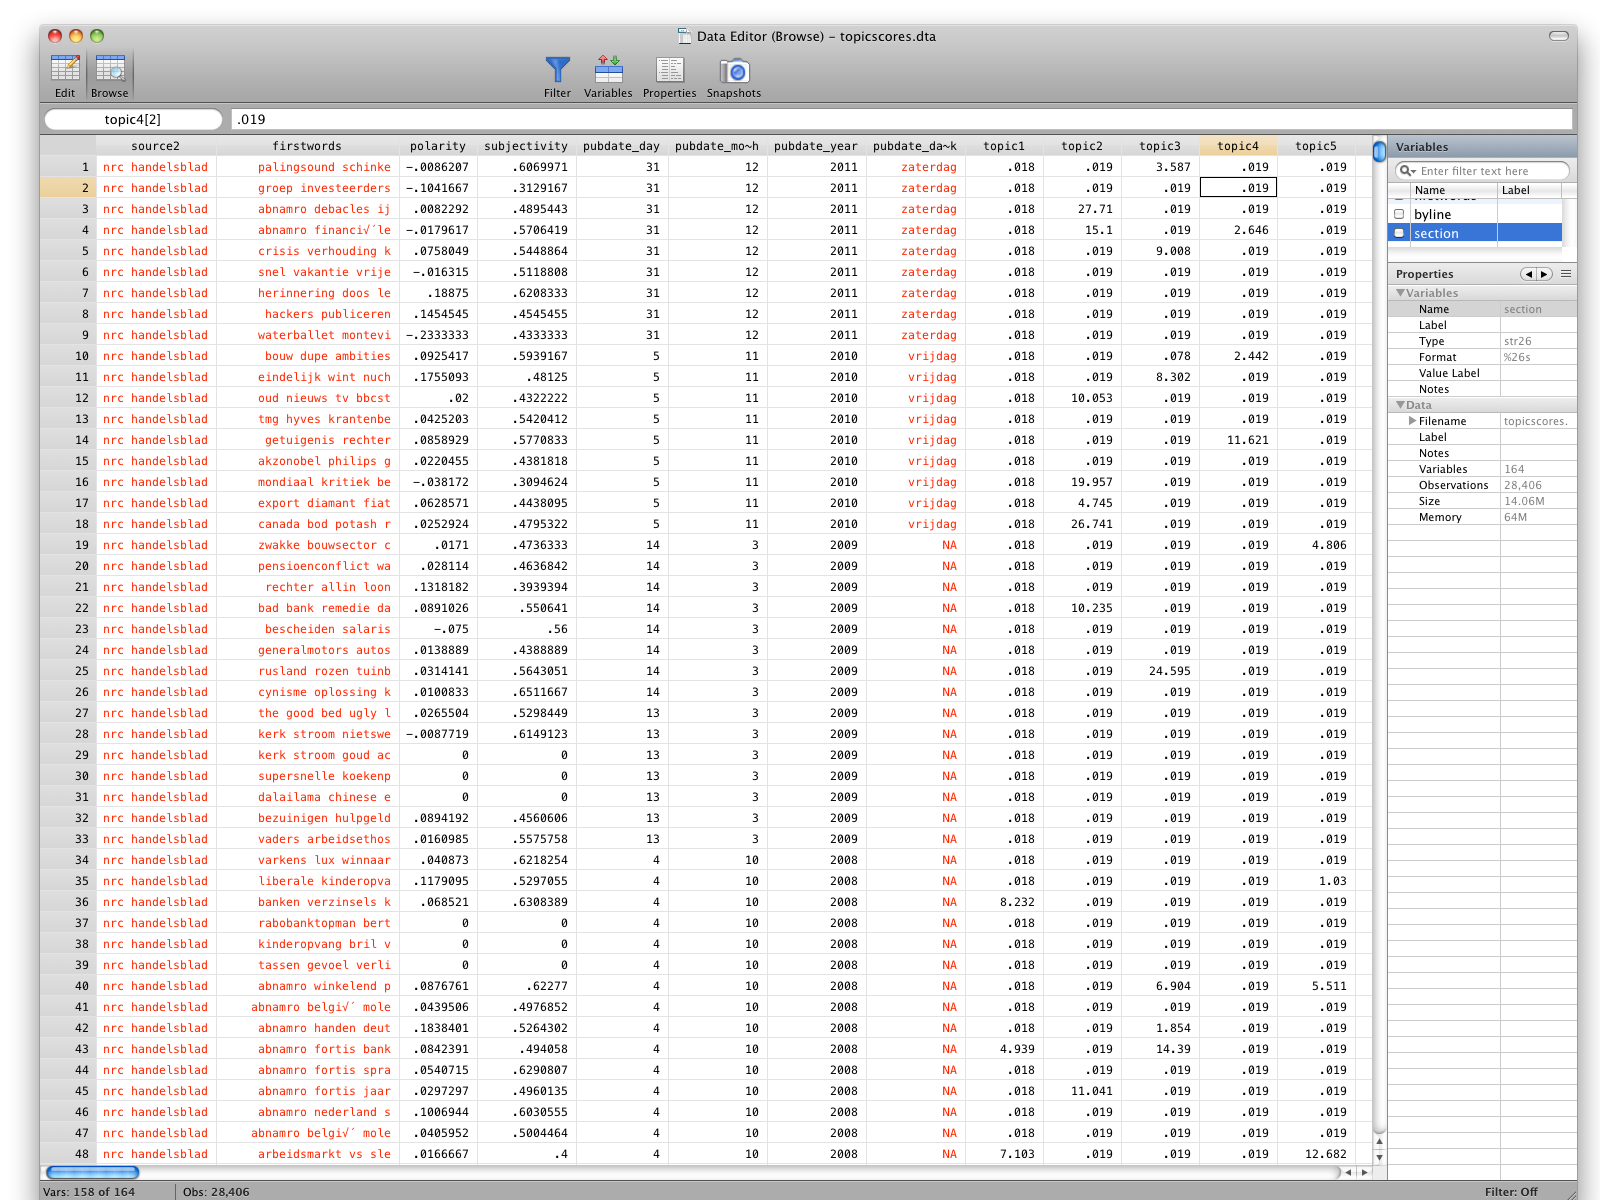
\includegraphics[width=\paperwidth,height=\paperheight,keepaspectratio]{topicscores}}
\end{frame}




\begin{frame}[fragile]{Visualization with pyldavis}
\begin{lstlisting}
import pyLDAvis
import pyLDAvis.gensim_models as gensimvis
# first estiate gensim model, then:
vis_data = gensimvis.prepare(mylda,mm,id2word)
pyLDAvis.display(vis_data)
\end{lstlisting}
\makebox[\linewidth]{
	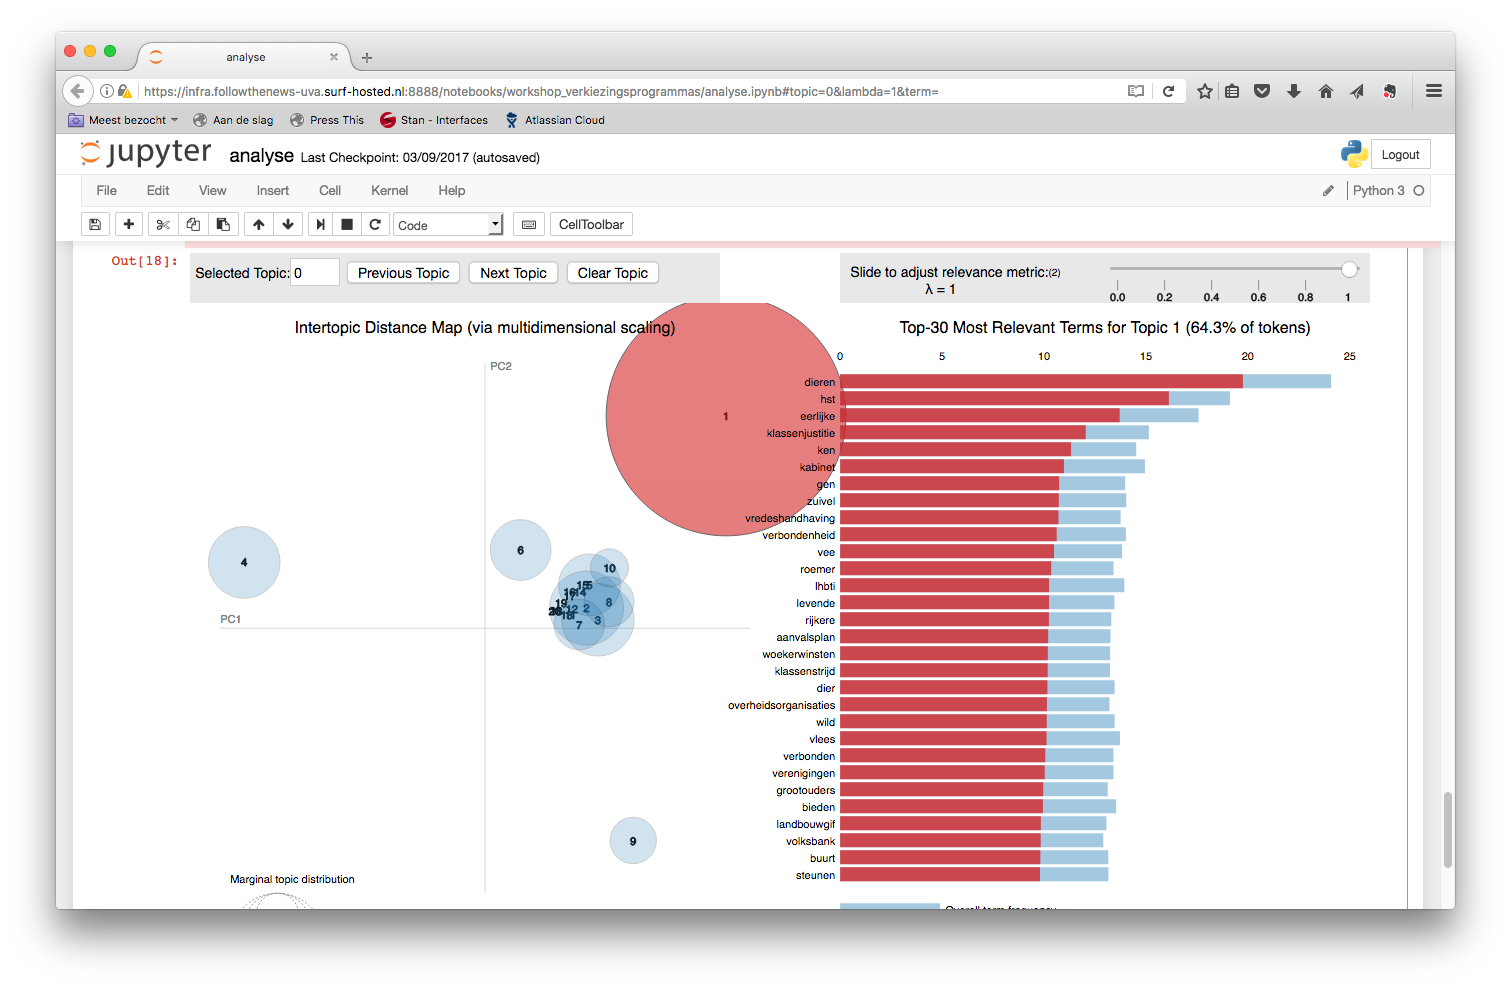
\includegraphics[width=\paperwidth,height=.5\paperheight,keepaspectratio]{pyldavis}}
\end{frame}

\begin{frame}{Visualization with pyldavis}
Short note about the $\lambda$ setting:

It influences the ordering of the words in pyldavis.

\begin{quote}
``For $\lambda = 1$, the ordering of the top words is equal to the ordering of the standard conditional word probabilities. For $\lambda$ close to zero, the most specific words of the topic will lead the list of top words. In their case study, Sievert and Shirley (2014, p. 67) found the best interpretability of topics using a  $\lambda$-value close to .6, which we adopted for our own case'' \parencite[p.~107]{Maier2018a}
\end{quote}

\end{frame}




\subsection{Choosing the best (or a good) topic model}

\begin{frame}{Choosing the best (or a good) topic model}
\begin{itemize}
\item There is no single best solution (e.g., do you want more coarse of fine-grained topics?)
\item Non-deterministic
\item Very sensitive to preprocessing choices
\item Interplay of both metrics and (qualitative) interpretability 
\end{itemize}

See for more elaborate guidance:

\tiny{Maier, D., Waldherr, A., Miltner, P., Wiedemann, G., Niekler, A., Keinert, A., \ldots Adam, S. (2018). Applying LDA Topic Modeling in Communication Research: Toward a Valid and Reliable Methodology. \textit{Communication Methods and Measures, 12}(2--3), 93--118. doi:10.1080/19312458.2018.1430754}

\end{frame}



\begin{frame}{Evaluation metrics (closer to zero is better)}
\begin{block}{perplexity}
A goodness-of-fit measure, answering the question: If we do a train-test split, how well does the trained model fit the test data?
\end{block}

\pause 
\begin{block}{coherence}
\begin{itemize}
\item mean coherence of the whole model: attempts to quantify the interpretability
\item coherence per topic: allows to get topics that are most likely to be coherently interpreted (\texttt{.top\_topics()})
\end{itemize}
\end{block}

\end{frame}


\begin{frame}{So, how do we do this?}
\begin{itemize}[<+->]
	\item Basically, similar to the idea behind our grid search from two weeks ago: estimate multiple models, store the metrics for each model, and then compare them (numerically, or by plotting)
	\item Idea: We select some candidate models, and then look whether they can be interpreted.
	\item But what can we tune?
\end{itemize}
\end{frame}


\begin{frame}{Choosing $k$: How many topics do we want?}
\begin{itemize}
	\item Typical values: $10<k<200$
	\item Too low: losing nuance, so broad it becomes meaningless
	\item Too high: picks up tiny pecularities instead of finding general patterns
	\item There is no inherent ordering of topics (unlike PCA!)
	\item We can throw away or merge topics later, so if out of $k=50$ topics 5 are not interpretable and a couple of others overlap, it still may be a good model
\end{itemize}
\end{frame}


\begin{frame}[fragile]{Choosing $\alpha$: how sparse should the document-topic distribution $\theta$ be?}
\begin{itemize}
	\item The higher $\alpha$, the more topics per document 
	\item Default: $1/k$
	\item But: We can explicitly change it, or -- really cool -- even learn $\alpha$ from the data (\texttt{alpha = "auto"})
\end{itemize}

\pause 

Takeaway: It takes longer, but you probably want to learn alpha from the data, using multiple passes:

\begin{lstlisting}
mylda LdaModel(corpus=tfidfcorpus[ldacorpus], id2word=id2word, num_topics=50, alpha='auto', passes=10)
\end{lstlisting}


\end{frame}


\begin{frame}{Choosing $\eta$: how sparse should the topic-word distribution $\lambda$ be?}
  \begin{itemize}
  \item Can be used to boost specific words
  \item Can also be learned from the data 
  \end{itemize}

\pause
Takeaway: Even though you can do \texttt{eta="auto"}, this usually does not help you much.

\end{frame}


% \subsection{Drawbacks of LDA topic models}


\subsection{Using topic models}

\begin{frame}{Using topic models}

You got your model -- what now?

\begin{enumerate}
\item Assign topic scores to documents
\item Label topics
\item Merge topics, throw away boilerplate topics and similar (manually, or aided by cluster analysis)
\item Compare topics between, e.g., outlets
\item or do some time-series analysis.
\end{enumerate}


Example: \cite{Tsur2015}

\end{frame}



\subsection{Other forms of topic models}

\begin{frame}{Other forms of topic models}
\begin{itemize}
\item Author-topic models
\item Structural topic models
\item Non-negative matrix factorization
\item \ldots
\end{itemize}
\end{frame}




